\section{Theoretical Analysis}
\label{sec:analysis}

In this section, the circuit shown in Figure~\ref{fig:circuit} is analysed
theoretically, in terms of its time and frequency responses.

\subsection{Mesh Analysis}

\begin{figure}
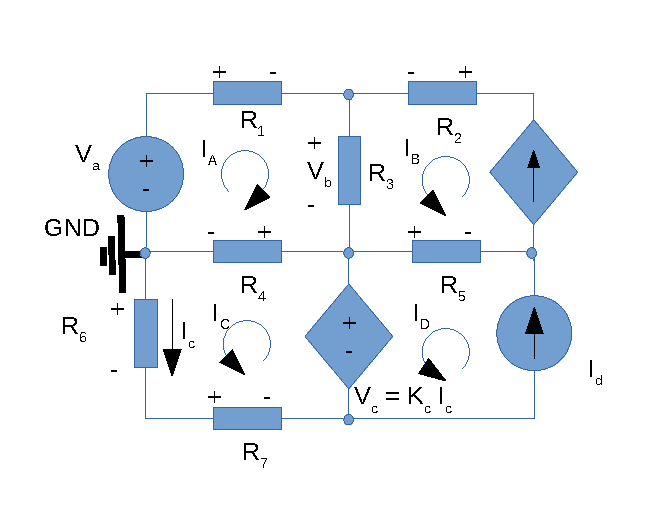
\includegraphics[width=0.4\linewidth]{circ_mesh.pdf}
\caption{Mesh Analysis}
\label{fig:circuitMesh}
\end{figure}

The Figure~\ref{fig:circuitMesh} has both the mesh's currents and the 
component's admited direction.
This reference is indispensable for the Nodal Analysis

\subsection{Nodal Analysis}

\begin{figure}
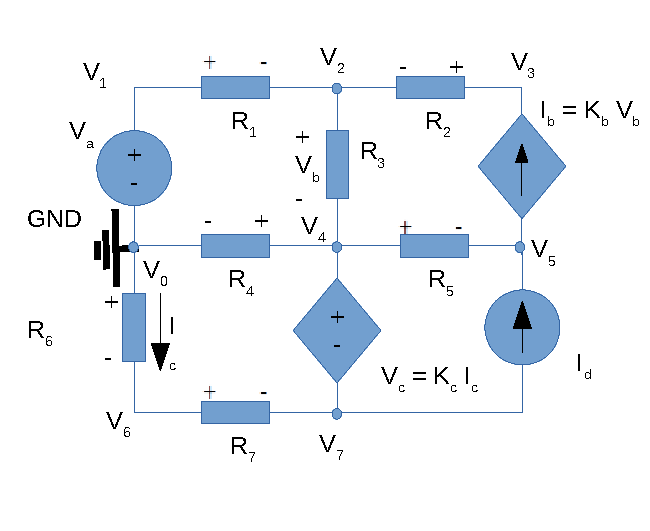
\includegraphics[width=0.4\linewidth]{circ_node.pdf}
\caption{Nodal Analysis}
\label{fig:circuitNodes}
\end{figure}

The Figure~\ref{fig:circuitNodes} has the node references added to it.
This reference is indispensable for the Nodal Analysis



